%
% Chapter 3
%

\chapter{DATA ANALYSIS} \label{chp:Analysis}

\section{Calibrations and Corrections}
In order to account for systematic errors inherent to the laboratory, several corrections and calibrations must be made to ensure proper $\gamma$-ray spectroscopy. A suite of in-beam ($^{24}$Na \& $^{60}$Co) and offline calibration ($^{226}$Ra \& $^{152}$Eu) sources were implemented during the experimental campaigns to provide the numerous corrections that must be made; successful calibration hinges on the implementation of a wide energy range of strong calibration lines that do not shift. An ADC nonlinearity, a detector efficiency, and a target sample self-absorption correction are all applied to energy calibrated spectra before the analysis of data can begin.

\subsection{Energy Calibrations}\label{sec:energy_calibrations}
Proper energy calibration is vital to the success of DSAM lifetime measurements; the precision in peak centroid location determines the sensitivity of the lifetime  measurement, as centroid energy shifts for longer-lived levels ($\sim$1~ps) can be as small as 20~eV. With its large range of energetic decays (from 185~keV to 2.4~MeV shown in Table \ref{tab:226Ralines}), $^{226}$Ra is an ideal candidate to energy calibrate our spectra; the $^{226}$Ra spectrum from the $^{162}$Dy(n,n$^\prime\gamma$) experiments can be seen in Figure \ref{fig:226Ra_spectrum}. Angular distribution measurements saw the presence of an in-line calibration source in the form of annular-shaped ring of $^{23}$Na that had been irradiated with a separate, on-site neutron source to produce radioactive $^{24}$Na. The $\beta$-decay to $^{24}$Mg$^*$ leads to a cascade of two intense $\gamma$-rays, 1368.626 and 2754.007~keV, providing a calibration point at a higher energy than a typical $^{60}$Co source can provide (1173.228 \& 1332.492~keV). This sodium ring is placed around the detector crystal to ensure the two calibration $\gamma$-rays are not attenuated by the passive shielding from the experimental setup shown in Figure \ref{fig:ExpSetup}. While far from an ideal candidate for an energy calibration point, radioactive $^{28}$Al from a $^{27}$Al(n,$\gamma$) channel will emit a high intensity $\gamma$-ray at 1778.785~keV; this peak originates from the aluminum housing for the HPGe detector and is often not well-defined in width, especially compared to the traditional Radium and Cobalt sources normally used, and as such, the $^{28}$Al should not be a main energy calibration point. A table of all online and offline calibrations used in the $^{160}$Gd and $^{162}$Dy experiments can be found in Table \ref{tab:calib_params}. 

\begin{landscape}
\begin{table}[ht]
% \centering
\begin{center}
\caption{CALIBRATION LINES: $^{226}$RA DECAY-CHAIN \label{tab:226Ralines}}

% $^{226}$Ra decays\\
% \makebox[\textwidth]{
\begin{tabular}{c|c||c|c||c|c||c|c}
\hline
E$_\gamma$ (keV) & I$_\gamma$ (rel) & E$_\gamma$ (keV) & I$_\gamma$ (rel) & E$_\gamma$ (keV) & I$_\gamma$ (rel) & E$_\gamma$ (keV) & I$_\gamma$ (rel)  \\
\hline \hline
186.053(4)  &  3.502(28)  & 487.090(70)  &  0.431(6)   & 1120.287(10) &  14.66(103) & 1661.280(60)  &  1.063(17) \\ \hline
241.997(3)  &  7.130(50)  & 580.130(30)  &  0.369(6)   & 1155.190(20) &  1.611(19)  & 1729.595(15)  &  2.791(22) \\\hline
258.870(40) &  0.525(5)   & 609.312(7)   &  44.83(314) & 1238.110(12) &  5.750(46)  & 1764.494(14)  &  15.03(105) \\\hline
274.800(50) &  0.472(6)   & 665.453(22)  &  1.506(12)  & 1280.960(20) &  1.411(16)  & 1847.420(25)  &  1.994(20) \\\hline
295.224(2)  &  18.09(127) & 768.356(10)  &  4.780(38)  & 1377.669(12) &  3.895(31)  & 2118.550(30)  &  1.137(11) \\\hline
351.932(2)  &  35.04(245) & 785.960(90)  &  1.097(12)  & 1385.310(30) &  0.782(9)   & 2204.210(40)  &  4.820(39) \\\hline
455.000(70) &  0.287(6)   & 806.174(18)  &  1.250(13)  & 1401.500(40) &  1.311(12)  & 2293.400(120) &  0.298(8) \\\hline
480.430(20) &  0.336(5)   & 934.061(12)  &  3.041(24)  & 1509.228(15) &  2.065(31)  & 2447.860(100) &  1.525(14) \\
\end{tabular}
% }\\ 
\vspace{10pt}
\end{center}
Energies (in keV) and relative intensities (in arbitrary units) for $\gamma$-ray emissions from the $^{226}$Ra decay chain used in data calibrations for this work.
\end{table}
\end{landscape}

\begin{figure}[ht]
\begin{center}
\includegraphics[width=0.95\textwidth]{calibration_226Ra.png}
\end{center}
\caption{Spectrum from a $^{226}$Ra calibration run during the $^{162}$Dy experiments. Sampled, higher intensity peaks are labeled by their energy in keV (refer to Table \ref{tab:226Ralines}).\label{fig:226Ra_spectrum}}
\end{figure}

\begin{landscape}
\begin{table}[ht]
% \centering
\begin{center}
\caption{ENERGY CALIBRATIONS: $^{160}$GD AND $^{162}$DY \label{tab:calib_params}} 

$^{160}$Gd(n,n$^\prime\gamma$) calibration E$_\gamma$ (keV)\\
% \makebox[\textwidth]{
\begin{tabular}{c|c|c|c|c|c|c}
\hline
\hline
E$_n$=1.5~MeV & 1173.228 & 1332.492  & 2223.245  \\ 
\hline
E$_n$=2.0~MeV &  1173.228 & 1332.492  & 2223.245    \\ 
\hline
E$_n$=2.8~MeV  &  1173.228 & 1332.492  & 1778.885 & 2223.245    \\ 
\hline
Excitation Function & 185.002 & 351.932 & 609.312 & 1120.287 &  1764.494 & 2223.245  \\ 
\end{tabular}
% }

\vspace{5mm}
% \centering
$^{162}$Dy(n,n$^\prime\gamma$) calibration E$_\gamma$ (keV)\\
% \makebox[\textwidth]{
\begin{tabular}{c|c|c|c|c|c|c|c|c}
\hline
\hline
E$_n$=1.6~MeV & 185.002 &  1173.228 & 1332.492 &  2223.245  \\ 
\hline
E$_n$=2.2~MeV & 185.002 &   1173.228 & 1332.492 &   2223.245    \\ 
\hline
E$_n$=3.1~MeV  & 351.932 & 609.312 & 1120.287 & 1173.228 & 1332.492 & 1764.494 & 2223.245 & 2754.007  \\ 
\hline
Excitation Function & 185.002 & 351.932 & 609.312 & 1120.287 &   1764.494 & 2223.245  \\ 
\end{tabular}
% }\\ 
\vspace{10pt}
\end{center}
Calibration points used for all $^{160}$Gd and $^{162}$Dy spectra energy calibrations, given in keV.
\end{table}
\end{landscape}

The linear energy calibrations from the $^{162}$Dy(n,n$^\prime\gamma$) experiments can be seen in figure \ref{fig:energy_calib}:

\begin{figure}[ht]
\begin{center}
\includegraphics[width=0.97\textwidth]{310_energy_calib.eps}
\caption{Linear energy calibration, taken from the three $^{162}$Dy(n,n$^{\prime}\gamma$) angular distributions and single excitation function (ExF in the legend).}
\label{fig:energy_calib}
\end{center}
\end{figure}

The difference in linear energy calibrations is the result of a change in gain settings between the two $^{162}$Dy experiments; the excitation function measurements and E$_n$=1.6 \& 2.2~MeV angular distributions occurred in August of 2013, while the single E$_n$=3.1~MeV angular distribution took place months later, in March of 2014. The specific difference in energy calibration can be seen in Figure \ref{fig:energy_calib}, where the electronics gain settings were changed (a natural, necessary, and sometimes unintentional occurrence in the laboratory). %The molar quantity of stable target material used in the DSAM experiments means we are not constrained by any natural radioactivity of the sample.

\subsection{Nonlinearity Calibrations}\label{sec:nonlinearity_calibration}
The first of these corrections is an ADC nonlinearity calibration, where a binning nonlinearity is introduced in the data acquisition's ADC. In the ideal case, an ADC correlates an analog voltage to a specific bin (in this case, the energy of a $\gamma$-ray on the absissca), with the bins being equally spaced and sized. We, of course, do not live in a perfect world, and some bins cover a larger energy range than others, generating an easily correctable error in the measurement of peak centroids. To perform this offline correction, a radioactive $^{226}$Ra source is placed at the same location the target is suspended, and is allowed to decay. Since the multitude of decays from $^{226}$Ra have very well defined and precise centroids, we can compare the measured position of these peaks to literature values for the peak centroids. By plotting a relationship between the change in channel as a function of energy, we can generate the specific nonlinearity curve to make the correction. Generally, the nonlinearity correction introduces a $\pm$2 channel difference (at most a 0.5~keV correction), and this nonlinearity can be fit to an order 5 polynomial, shown in Figure \ref{fig:dsnonlin}:

\begin{figure}[ht]
\begin{center}
\includegraphics[width=0.97\textwidth]{310_dsnonlin_color.eps}
\caption{Order-5 polynomial nonlinearity correction, taken from the $^{162}$Dy(n,n$^{\prime}\gamma$) angular distribution with E$_n$=3.1~MeV}
\label{fig:dsnonlin}
\end{center}
\end{figure}
Special care must be taken to ensure a realistic polynomial fit for the ADC nonlinearity; polynomials of high order can gravely mis-characterize the ADC behavior outside of the range of calibration points used (in our case, $^{226}$Ra decays). In Figure \ref{fig:dsnonlin}, the downward turn in the fifth-order extrapolation above 2.5~MeV $\gamma$-rays would be magnified for higher order odd polynomials, and would turn upward (at a similarly unrealistic rate) for the even polynomials. To justify the use of an order-5 polynomial, the highest energy $\gamma$-ray observed in the $^{162}$Dy experiments is a 2779~keV de-excitation, keeping in line with a $\sim\pm$1~keV nonlinearity correction.
\subsection{Efficiency Calibrations}\label{sec:efficiency_calibration}
High Purity Germanium detectors have an intrinsic detection efficiency, dependent on the energy of a particular $\gamma$-ray that enters the Ge crystal; higher energy $\gamma$-rays have a lower probability of depositing their entire energy into the detector, so this must be accounted for in angular distribution data to get correct $\gamma$-ray intensities. The same spectrum from the nonlinearity calibrations is used, as we can simply compare the measured intensities of $\gamma$-rays from the $^{226}$Ra source to the literature values of $\gamma$-ray intensity. This efficiency correction is shown in Figure \ref{fig:polyfit} as a function of \textit{E$_\gamma$}:

\begin{figure}[ht]
\begin{center}
\includegraphics[width=0.97\textwidth]{310_polyfit_color.eps}
\caption{Fifth-order relative efficiency curve taken from the $^{162}$Dy(n,n$^{\prime}\gamma$) angular distribution with E$_n$=3.1~MeV
\label{fig:polyfit}}
\end{center}
\end{figure}

\subsection{Self-Absorption Corrections}\label{sec:gambit_correction}
One of the key characteristics of the Winterbon formalism for determining \textit{F}(\textit{$\tau$}) as a funciton of \textit{$\tau$} is the use of large quantities of target material to provide sufficient nuclear and electronic stopping power \cite{WINTERBON_1975}. Of course, a downside to using these molar quantities of powder targets is that incoming neutrons and outgoing $\gamma$-rays will be attenuated by the physical thickness of material. Much like the efficiency calibration, the self-absorption correction must be made to get proper $\gamma$-ray intensities, since low-energy gamma rays may be drastically attenuated by the thickness of the sample. Both the physical geometry of the experimental setup and size of the sample affect this highly-angular dependent correction, used solely in the angular distribution data in the presented analysis. The {\tt GAMBIT} (\cite{ENGELBRECHT1970187}, \cite{CONTE_NUMERICAL_text}, \cite{GAMBIT_BORING1960}) codes and subroutines are well-equipped to perform this correction for any experiment performed at UKAL involving a cylindrical target cell; {\tt GAMBIT} takes into account differential elastic neutron cross sections (\textit{$\frac{d\sigma_n}{d\Omega}$} at 0$^\circ$ and 180$^\circ$), total neutron cross sections ($\sigma_{n,\textit{tot}}$), elastic neutron scattering cross sections ($\sigma_{n,\textit{el.}}$), and the photon absorption cross sections ($\sigma_{\gamma}$ for each composite material found in the sample ($^{162}$Dy$_2^{16}$O$_3$). Figure \ref{fig:gambit} shows the multiplicative factor needed to give the correct peak areas from this self-absorption of $\gamma$-rays as a function of $\theta_{lab}$. Factors near unity indicate little to no correction is needed (at higher energies, a $\gamma$-ray can easily escape the physical target), while a significant correction must be made to low-energy ($<$200 keV) $\gamma$-rays that are partially or heavily attenuated by the sample. 

\begin{figure}[ht]
\begin{center}
\includegraphics[width=0.97\textwidth]{gambit.eps}
\caption{Multiplicative factor calculated by {\tt GAMBIT} to correct for the angular dependent $\gamma$-ray self-absorption by a finite-size target. \label{fig:gambit}}
\end{center}
\end{figure}

This self-absorption correction given by {\tt GAMBIT} is sufficient and appropriate for use in the (n,n$^\prime\gamma$) experiments at UKAL, even though much more modern approaches to characterize the self-absorption exist. Molecular dynamics calculations can be made to generate this angularly and energetically dependent attenuation, but require a much higher amount of computational power to complete. Since the newer, refined methods do not offer a more efficient or accurate self-absorption calculation, we can confidently use the more simplistic approach given by the {\tt GAMBIT} code.

\section{Statistical Analysis}
The wealth of information that can be extracted from $\gamma$-ray spectroscopy hinges on consistent, precise statistical analysis of spectra. An example of a properly TOF gated, energy calibrated, and background subtracted spectrum can be seen in Figure \ref{fig:examplespec}:

\begin{figure}[h]
\begin{center}
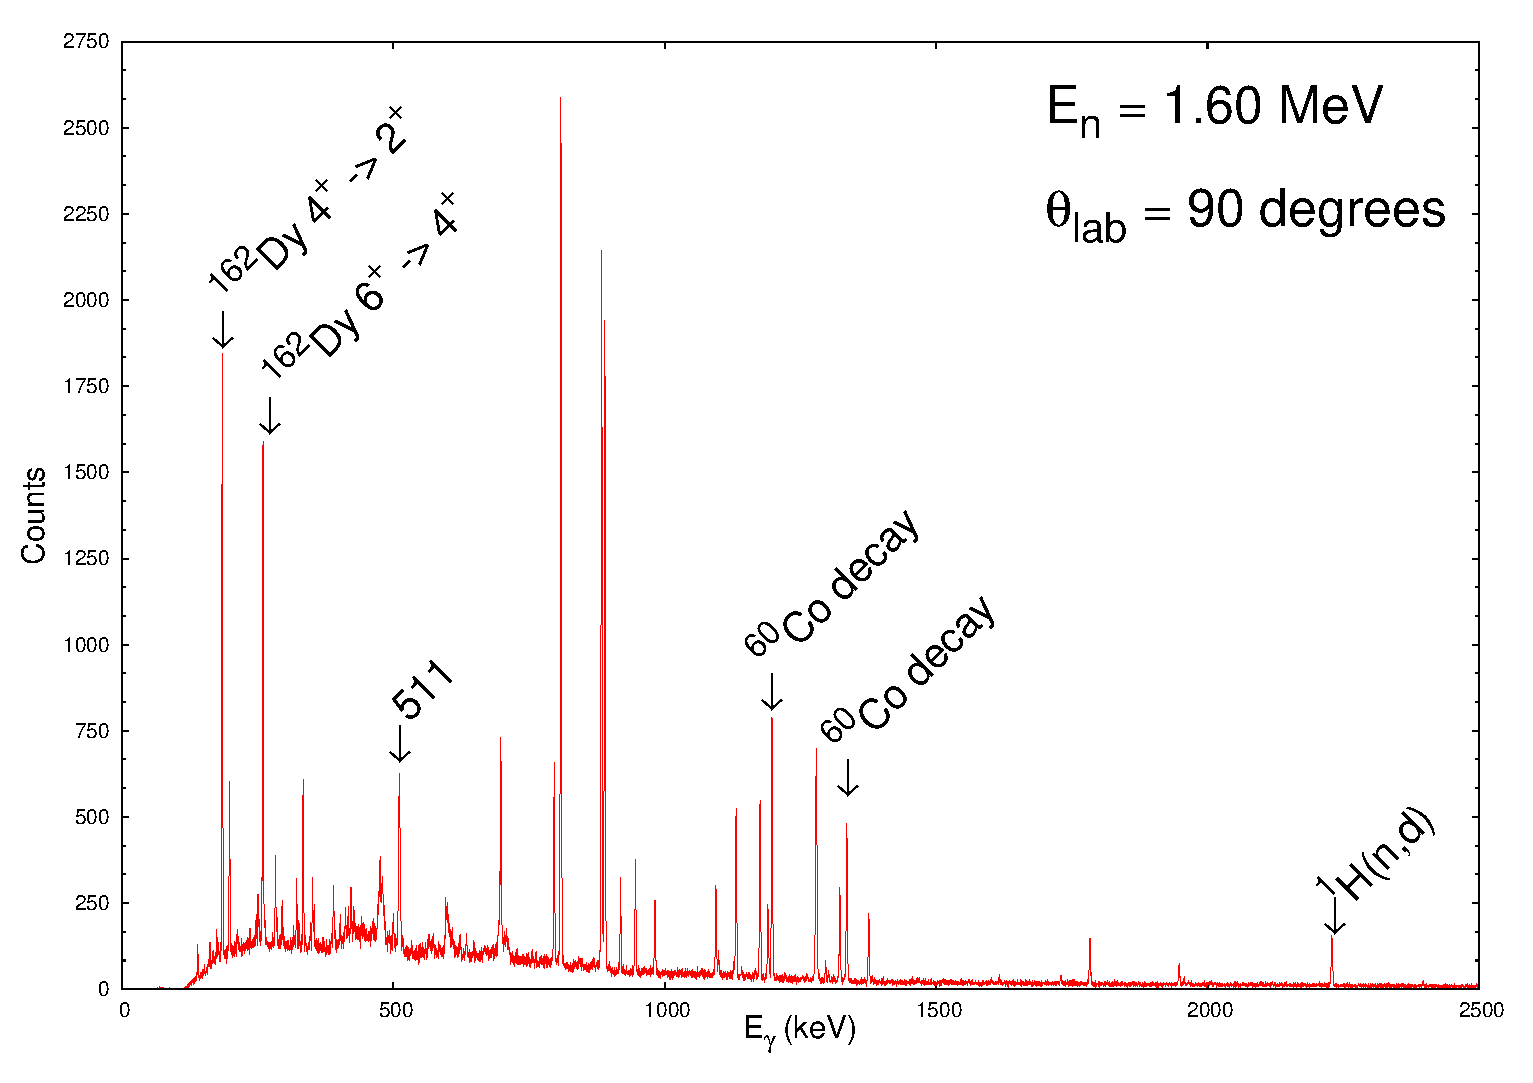
\includegraphics[width=0.95\textwidth]{samplespec.eps}
\caption{Example of an energy-calibrated spectrum from the $^{162}$Dy angular distribution at E$_n$=1.6~MeV and $\theta_{lab}$=90$^\circ$, outlining typical background levels and miscellaneous $\gamma$-ray transitions.
\label{fig:examplespec}}
\end{center}
\end{figure}

\subsection{Fitting Procedures}\label{sec:fitting_procedures}
A $\gamma$-ray event recorded in the HPGe detector will manifest itself as a skewed, defined-width gaussian distribution on the histogram of the form shown in Equation \ref{eq:gaussian}, and is fit according to:

\begin{equation}\label{eq:gaussian}
y=\sum_k \frac{A_k}{(2\pi)^\frac{1}{2}\sigma}e^{-\frac{1}{2}\left(\frac{Z-Z_k}{\sigma}\right)^2}\left[1+P_{left,1}\left(\frac{Z-Z_k}{\sigma}\right)^4+P_{left,2}\left(\frac{Z-Z_k}{\sigma}\right)^{12}\right]
\end{equation}

The multiple parameter fitting procedure in Equation \ref{eq:gaussian} can be qualitatively described as measures of \textit{$\sigma$}, the width of the peak, \textit{Z$_k$}, the centroid location of a peak, \textit{A$_k$}, the peak height, and two parameters relating to the low-energy tail (a measure of the skewedness of the gaussian), \textit{P$_{left,1}$} \& \textit{P$_{left,2}$}. This trailing edge is the result of Bremsstrahlung escape from the detector itself \cite{Knoll_text}, but is necessary to accurately fit low-intensity peaks that exist as a doublet with higher-intensity peaks. For a given peak, three parameters are interpolated separately into a $\chi^2$ fit, the width, $\sigma$, and the two left-polynomial terms, \textit{P$_{left,1}$} \& \textit{P$_{left,2}$}. Typically, the polynomial terms are a small, but significant contribution (\textit{P$_{left,1}$}$<$0.010), and $\sigma$ is bounded between $\sim$2 and $\sim$7 channels ($\sim$0.5 to $\sim$1.5~keV energy resolution). These open parameters are iteratively fit one at a time to best recreate the shape of the gaussian distribution in the histogram; once all peaks have been properly fitted, the fit parameters are exported to a peak list with peak areas, centroids (subsequently the energy of the $\gamma$-ray), and the associated statistical errors from each parameter. \textit{F$_i$tP$_i$c} \cite{FitPic_Fribourg} was used to interpolate fit parameters for all experimental data in both $^{160}$Gd and $^{162}$Dy. Peaks are assigned to groups with up to five other peaks to ensure a locally linear background for each gaussian. 
\subsection{Observable Extraction}
From the peak list, we can extract a wealth of knowledge about the decay radiation observed, even with the seemingly basic information gained from fitting the peaks in a given histogram.
\subsubsection{Excitation Functions}\label{sec:excitation_functions}
Although no direct measurable quantities ($\gamma$-ray energies, branching ratios, etc) can be extracted from the excitation function data, previously unplaced $\gamma$ rays can be assigned to de-exciting levels simply by looking at the raw threshold of $\gamma$-ray population. Two plots per $\gamma$-ray are generated, the relationship between E$_\gamma$ and E$_n$, and peak area as a function of E$_n$; the first plot allows confirmation that each peak is fit uniformly, where the relationship between peak area and neutron energy will allow us to determine an approximate threshold energy. Any modulation of the $\gamma$-ray energy as a function of bombarding neutron energy is a signature of non-uniform peak fitting or that another $\gamma$-ray of similar energy has been populated in the level scheme at a different threshold. When this latter case occurs, the peak area as a funciton of neutron energy will also show a corresponding bump at the same threshold. An example of this ensemble of plots is shown in Figure \ref{fig:sample_exf}:


\begin{figure}[h!]
\begin{center}
\includegraphics[width=0.97\textwidth]{sample_exf.eps}
\caption{A set of plots from a typical excitation function for a single $\gamma$-ray transition, in `a)', E$_\gamma$ vs. E$_n$, and in `b)', the peak area vs E$_n$. Note the dip in $\gamma$-ray energy at 2.6~MeV, and corresponding bump in peak area (shown as a blue ellipse to guide the eye), indicating a second transition of a similar (slightly lower) energy being populated.
\label{fig:sample_exf}}
\end{center}
\end{figure}

The absolute threshold energies for $\gamma$-rays are used to determine where a $\gamma$-ray comes in, and to determine which level is providing the de-excitation, a problem that would otherwise require $\gamma$-$\gamma$ coincidence measurements. Since the excitation functions give $\gamma$-ray placements in the nucleus, we are no longer reliant on the more complex coincidence measurements. 

Figure \ref{fig:ExF_difference_140_230} shows an example of the population rate of a $\gamma$-decay in $^{162}$Dy by superimposing multiple neutron energy spectra on top of each other. Take note that the E$_n$=1.4 and 1.7~MeV datasets are below the energy threshold of the level that the 1647~keV decay leaves, with a sharp increase of counted statistics just above the level energy threshold, growing until a well-defined gaussian peak is seen at E$_n$=2.3~MeV.

\begin{figure}[h!]
\begin{center}
\includegraphics[width=0.97\textwidth]{ExF_difference_140_230.eps}
\caption{Spectra from four bombarding neutron energies (E$_n$=1.4, 1.7, 1.775, and 2.3~MeV datasets) to show the typical increase of statistics for a single peak, a 1647~keV decay from the 1728~keV state in $^{162}$Dy. Note the peak area emerge just above the level energy threshold (1.775~MeV neutron dataset), with optimal statistics in the E$_n$=2.3~MeV set.
\label{fig:ExF_difference_140_230}}
\end{center}
\end{figure}

Proper placement of $\gamma$-rays in the level scheme is vital to confident, precise measurement of level lifetimes, absolute intensities, and multipole mixing fractions. Although the experiments at UKAL are not designed to find new J=0 states (\textit{e.g.} something the Q3D spectrometer can better achieve with two nucleon transfer reactions), tentative spin assignments and/or confirmation of spin can be placed with information from both the excitation functions and angular distributions. J=0 excitations should have a threshold very close to the energy of the state, as there is very little angular momentum needed to populate the state, and since inelastic neutron scattering can only realistically populate up to spin 5$^\pm$ states (a consequence of the limited angular momentum transfer from the spin-$\frac{1}{2}$ neutron to the nucleus during inelastic scattering), stringent upper limits on the spin and parity of a parent level can be placed by examining the spin and parity of the daughter state. For example, if a transition between two levels is energetically feasible, we know that the spin and parity of the parent state will be within $\pm$2 units of angular momentum of the daughter level because only $\Delta$J$<$2 multipolarities are observed in the laboratory with any appreciable or measurable intensity, as the relative intensity of E3, E4 and higher multipolarities are orders of magnitude less intense than the strong E2 quadrupole radiation observed in the lab.  For example, in cases where the daugher level is spin-5, we know that the parent state will be spin-3 or spin-4, due to the low spin-population of inelastic neutron scattering. 

%[ENERGY THRESHOLDS TO PLACE UNASSIGNED GAMMA RAYS]
\subsubsection{Angular Distributions}\label{sec:AD_Ft}
Spectra from the angular distributions have all corrections applied (nonlinearity, detector efficiency, and self-absorption), where the peak list is separated and sorted into groups based on the $\gamma$-ray energy as a function of angle. Careful bounding of groups must be made to ensure good $\gamma$-ray separation in the event of a close-lying doublets, while maintaining sufficient overhead to account for large-order Doppler energy shifts (very short lifetimes on the order of $\sim$10~fs). 

%[TALK ABOUT ACTUAL CALCULATION OF F($\tau$) factor]
In order to extract the lifetime of a particular state, precise calculation of the theoretical values for \textit{F}(\textit{$\tau$}) (Winterbon curve) must be made to compare the extracted \textit{F}(\textit{$\tau$}) from the Doppler shifted $\gamma$-rays. This calculation is achieved via {\tt v1pgm}, which takes into account the calculated recoil velocity from Equation \ref{eq:betarecoil}, the target density and atomic weight of each element in the target, and a range of lifetimes to iterate over (from 1~fs to 10~ps). Since the target does not change composition or density, the only input parameter that changes is the nuclear recoil velocity, dependent solely on the bombarding neutron energy. The calculated Winterbon curves for the $^{162}$Dy experiments can be seen in Figure \ref{fig:ftau_all}, with an emphasis to highlight the ideal range ($\sim$10~-~$\sim$600~fs) to measure lifetimes with DSAM. In general, \textit{F}(\textit{$\tau$}) is constrained by the uncertainties in electronic and nuclear stopping powers, resulting in $\sim$10\% uncertainty in the attenuation factor \cite{Belgya_DSAM1996}; this uncertainty is propagated to the extracted lifetime's uncertainty.

\begin{figure}[ht]
\begin{center}
\includegraphics[width=0.97\textwidth]{ftau_all.eps}
\caption{Calculated Winterbon curves (\textit{F}(\textit{$\tau$}) as a function of \textit{$\tau$}) for E$_n$=1.6, 2.2, and 3.1~MeV $^{162}$Dy angular distributions. Sensitive lifetime ranges from DSAM are shown as vertical black lines, with the corresponding \textit{F}(\textit{$\tau$}) values as horizontal lines.
\label{fig:ftau_all}}
\end{center}
\end{figure}

Direct comparison of the experimental \textit{F}(\textit{$\tau$}) value to the calculated Winterbon curve for a particular $\gamma$-ray is straightforward; in Figure \ref{fig:DSAM_example}, the measured slope of the Doppler shift of 0.665 correlates to a \textit{$\tau$} of 21~fs. For excited states with only one de-exciting transition, the extracted $\gamma$-ray lifetime is equivalent to the level lifetime, where level lifetimes with multi-channel $\gamma$-ray de-excitations are extracted from the weighted average of all de-exciting \textit{F}(\textit{$\tau$}) values, weighted by the uncertainty in each measured F($\tau$). This standard statistical average can be explicitly seen in Equation \ref{eq:weighted_average} taken from \cite{Bevington_text}. Special care must be taken, however, to ensure accurate and precise Doppler shifts are obtained from the various de-excitation channels from a level. In several cases for low energy and/or intensity $\gamma$ rays, the shift (magnitude of F($\tau$)) will be negative or consistent with zero; in this case, any lifetime deduced from the Doppler shift is not accounted in the weighted average of the level lifetime. The same rules apply when a particular $\gamma$ ray has the potential to be coincident with a background line, where the F($\tau$) value may be unreliable. As a rule of thumb, F($\tau$) should be about 1$\sigma$ variance from zero to be considered a good candidate for DSAM, however, this is sometimes impossible if the physical lifetime is on the precipice of the sensitive range of lifetimes DSAM can measure. Large upper uncertainties are not uncommon for the near-picosecond lifetimes with `shallow' values for F($\tau$) measured with DSAM (e.g. 3000$^{+4800}_{-1300}$~fs for the 1666~keV state in $^{162}$Dy), yet another experimental challenge we must overcome when measuring the lifetimes of states.

\begin{equation}\label{eq:weighted_average}
\widehat{F(\tau)}=\frac{\sum_{i} F_i(\tau) \sigma^{-2}_i}{\sum_{i}\sigma^{-2}_i}, \sigma^2(\widehat{F(\tau)})=\frac{1}{\sum_i \sigma^{-2}_i}
\end{equation}

\begin{figure}[ht]
\begin{center}
\includegraphics[width=0.97\textwidth]{DSAM_example.eps}
\caption{Example Doppler Shift for a 1149~keV $\gamma$-ray populated in the 1.5~MeV $^{160}$Gd(n,n$^\prime\gamma$) experiment. Here, the \textit{F}(\textit{$\tau$}) value of 0.665 $\pm$ 0.010 corresponds to a lifetime of 21 $\pm$ 1 fs.
\label{fig:DSAM_example}}
\end{center}
\end{figure}

Further refinement of any spin assignments made in the literature can be deduced by examining the a$_2$ and a$_4$ coefficients from Equation \ref{eq:angdistW}; isotropic or near-isotropic angular distributions could suggest significant multipole mixing of $\gamma$ radiation, as pure E2, E1, or M1 radiation will mimic the classical radiation patterns displayed in Figure \ref{fig:multipole_diff}. The decay radiation pattern leaving a 0$^+$ excitation will also be isotropic in the angular distribution, as this is the equivalent of an unaligned decaying state. The angular distributions can be used to confirm or deny tentative spin-0 states by examining the angular distribution, but this technique should not be used to find new 0$^+$ excitations (two nucleon transfer reactions are still a much higher resolution method). For all angular distributions presented in this work, the peak areas are normalized in a way to ensure the angular distribution of the decay from the first excited 0$^+$ state is isotropic (a$_2$ consistent with 0). This is justified in \cite{Lesher_160Gd0s}, where multiple angular distribution normalizations were examined: once with the above normalization, and once where we normalized the peak area to another tentative (now repudiated) 0$^+$ state with disastrous results. Under this secondary normalization, strong E2 transitions that show no mixing ceased to have the same qualitative shape of a pure quadrupole in Figure \ref{fig:multipole_diff}, implying this was not a suitable candidate for normalization (or as an isotropic 0$^+$ $\rightarrow$ 2$^+$ transition). Special care must also be taken with the evaluation of the angular distributions, as there are multiple ways to create an isotropic distribution, via proper mixing of multipole radiation (admixtures of E2 and M1 radiation).

If the angular distribution is not isotropic or indicative of a pure quadrupole or dipole radiation (Figure \ref{fig:multipole_diff}), then the $\gamma$-ray may be of a mixed multipolarity. This commonly occurs in transitions where J$^\pi_i$ $\approx$ J$^\pi_f$, but is not to be confused with an E0 monopole transition, which is strictly forbidden by $\gamma$ decay and must occur via internal conversion electrons. In order to characterize this mixing, we compare the a$_2$ and a$_4$ coefficients to theoretical calculations of the same a$_2$ and a$_4$ coefficients for a particular J$^\pi$ value for a level, assuming there is no mixing. The statistical model for a compound nucleus is used to calculate cross sections for a (n,n$^\prime\gamma$) reaction with the target nucleus being treated as an optical model potential (the combination of a real Woods-Saxon potential with a diffuse, imaginary Gaussian surface potential). The {\tt FORTRAN} code used to achieve this calculation is {\tt CINDY} (a Hauser-Feschbach formalism taken from \cite{SHELDON197399}). The multipole mixing fraction (effectively a$_2$ and a$_4$) is then varied in the statistical model to reproduce the angular distribution for a possible J$^\pi$; the direct comparison of experimental Legendre Polynomial coefficients to those calculated in this statistical model lead directly to $\chi^2$ as a function of $\delta$, the multipole mixing fraction. Any $\gamma$-ray observed in our experiments that has a known placement in the level scheme can be added to the optical model to perform this $\chi^2$ minimization, where the smallest value of $\chi^2$ corresponds to the optimal value of $\delta$ for a particular de-excitation. These experimental mixing fractions aid in the calculation of the reduced transition probabilities for mixed multipolarity $\gamma$ decays given in Equation \ref{eq:BE2exp}, also using Equations \ref{eq:FE2} or \ref{eq:FM1}. An example extraction of $\delta$ from the angular distribution of $\gamma$-rays can be seen in Figure \ref{fig:delta_mixing_example}; $\chi^2$ is minimized locally for this $\gamma$ ray at a $\delta$ value $\sim$1, which indicates $\sim$50\% E2/M1 mixing. In Figure \ref{fig:delta_mixing_example}, the top left plot shows the measured angular distribution of the 1308~keV $\gamma$ ray, with {\tt CINDY} calculations for a range of starting spins decaying to a spin-4 state. The intersection of the black ellipse and the colored ellipses (calculations) correspond to the projections in the bottom plot, where we verify the lowest $\chi^2$ value on the y-axis for a particular delta on the x-axis for the 4$^+\rightarrow$4$^+$ transition.

\begin{figure}[ht]
\begin{center}
\includegraphics[height=0.25\textheight]{1308_AD_fit.png}
\includegraphics[height=0.25\textheight]{1308_AD_chisq_fit.png}\\
\includegraphics[width=0.73\textwidth]{1308_AD_delta_chi.png}\\
\caption{Example extraction of multipole mixing fraction ($\delta$) for a 4$^+\rightarrow$4$^+$ transition in $^{162}$Dy. Top-left plot: angular distribution of the 1308~keV $\gamma$ ray. Top-right plot: {\tt CINDY} comparison for a range of initial spins (color online) decaying to the final spin of 4; intersections with the black ellipse mark local/global minima of $\chi^2$ vs $\delta$. Bottom plot: projection of {\tt CINDY} comparison as $\chi^2$ as a function of $\delta$ minimization (note the lowest $\chi$ value corresponds to the $\delta\approx$1 for the cyan-colored 4$^+\rightarrow$4$^+$ transition). (color online) \label{fig:delta_mixing_example}}
\end{center}
\end{figure}
%add in an example figure of mixing and the chi squared minimzation process????
%possibly add in U=V+iW

To round out the cadre of important experimental information, we can extract the absolute intensity of $\gamma$-rays that de-excite the nucleus from the angular distribution data. The \textit{A$_o$} coefficient from Equation \ref{eq:angdistW} is proportional to the absolute intensity, and simply needs to have the efficiency \& self-absorption corrections applied to the measured \textit{A$_o$} (gross peak area). The branching ratios immediately follow from the absolute intensities, since we know all $\gamma$-decay channels open to a particular level, and these are used to calculate absolute transition probabilities (Equation \ref{eq:BE2exp}).


